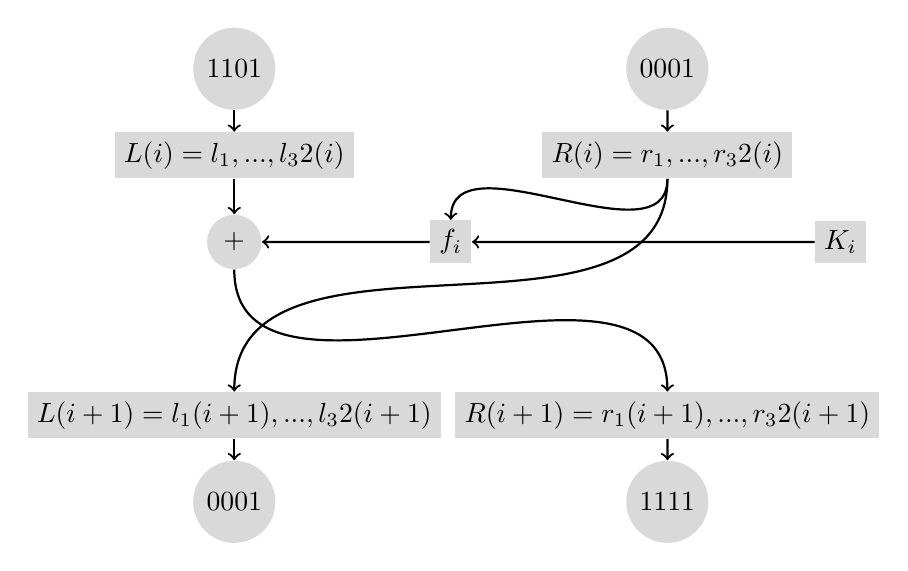
\begin{tikzpicture}[scale=1.1]
  \node [circle, fill=gray!30] (c1) at (0, 0) {$ 0001 $};
  \node [circle, fill=gray!30] (c2) at (5, 0) {$ 1111 $};
  \node (a1) at (0,1) [fill=gray!30] {$L(i+1)=l_1 (i+1), ... ,l_32(i+1)$};
  \node (a2) at (5,1) [fill=gray!30] {$R(i+1)=r_1 (i+1), ... ,r_32(i+1)$};
  \node (a3) at (0,4) [fill=gray!30] {$L(i)=l_1 , ... , l_32 (i)$};
  \node (a4) at (5,4) [fill=gray!30] {$R(i)=r_1 , ... , r_32 (i)$};
  \node [circle, fill=gray!30] (c3) at (0, 5) {$ 1101 $};
  \node [circle, fill=gray!30] (c4) at (5, 5) {$ 0001 $};
  \node [circle, fill=gray!30] (c5) at (0, 3) {$ + $};
  \node (a5) at (2.5,3) [fill=gray!30] {$f_i$};
  \node (a6) at (7,3) [fill=gray!30] {$K_i$};

  \draw[->, thick] (c3) to (a3);
  \draw[->, thick] (c4) to (a4);
  \draw[->, thick] (a3) to (c5);
  \draw[->, thick] (a1) to (c1);
  \draw[->, thick] (a2) to (c2);
  \draw[->, thick] (a6) to (a5);
  \draw[->, thick] (a5) to (c5);
  \draw[->, thick] (c5) to[out=-90, in=90] (a2)  ;
  \draw[->, thick] (a4) to[out=-90, in=90] (a1)  ;
  \draw[->, thick] (a4) to[out=-90, in=90] (a5)  ;
\end{tikzpicture}
